\scanpage{214}
% archive sheet number: 213

\diagram{\begin{tikzcd}[ampersand replacement=\&,column sep=large,row sep=small]
\deleted{X^P}\arrow[r,hook,"\deleted{\alpha_P}","{\text{\deleted{imm. fermée}}}"']\arrow[d]\&\deleted{X^E}\\
\deleted{F_P}\&
\end{tikzcd}}

\[
\deleted{X^E=\bigcup_{\substack{P\\\text{(disjointe)}}}\alpha_P((X^P)^*)}
\]

\[
\deleted{(f^E)^{-1}(\Delta_Y^{(E)})=\bigcup_{\substack{P\\\text{somme}\\\text{disjointe}}}
\underbrace{\alpha_P(F_P)}_{\substack{\text{de dim }n-(\operatorname{card}P-1)d\,\geq\,n-\operatorname{card}(E)d\\
\text{égalité pour }P=\underbrace{P_0}_{\text{partition maximale}}\text{ seulement}}}}
\]

\[
\begin{aligned}
&\deleted{\underline{\operatorname{Card}} E=3} &\deleted{\text{partition en }3:P_0}\\
&&\deleted{\text{partitions en }2:(1)(23),(2)(31),(3)(12)}\quad\deleted{P_{23}\quad P_{31}\quad P_{12}}\\
&&\deleted{\text{partition en }3:P_1}
\end{aligned}
\]

\[
\deleted{(f^3)^{-1}(\Delta_Y^{(3)})=
\underset{n-2d}{F_3}\ \cup\!
\bigcup_{1\leq i<j\leq 3}\underset{n-d}{\alpha_{ij}(F_2)}\ \cup\
\underset{n}{\Delta_X^{(3)}}}
\]

\deleted{dim ``génériques''}

\deleted{\uline{Question}}

\[
\begin{aligned}
&\deleted{\overline F_3\cap\Delta_X^{(3)}=\emptyset}\\
&\deleted{\overline{\alpha_{ij}(F_2)}\cap\Delta_X^3=\alpha_{ij}(\overline F_2)\cap\Delta_X^{(3)}
=\alpha_{ij}(\underbrace{\overline F_2\cap\Delta_X^{(3)}}_{\substack{=\emptyset\ \text{si}\\f\ \text{\unsure{net}}}})=\boxed{\emptyset}}\\
&\deleted{\overline F_3\cap\overline{\alpha_{ij}(F_2)}\unsure{\mathord{\cdot}|=|,}\overline F_3\cap\alpha_{ij}(\overline F_2)}
\end{aligned}
\]

\deleted{\uline{NB} Si $f$ net, alors $\overline F_3\cap\underset{\text{fermé}}{\Delta_X^{(3)}}=\emptyset$, $\overline{\alpha_{ij}(F_{\unsure{1|2}})}\cap\Delta_X^{(3)}=\emptyset$}

\deleted{Mais que peut-on dire de}

\[
\deleted{\overline F_3\cap\overline{\alpha_{ij}(F_2)}\mathord{\cdot}\overline F_3\cap\alpha_{ij}(\overline F_2)}
\]

\[
\deleted{\underbrace{x_1^{\unsure{\lambda|d|0}}\ne x_2^\lambda\ne x_3^\lambda}_{\ne}}
\qquad \underbrace{x_1^0=x_3^0}\ne x_2^0
\]

\figure{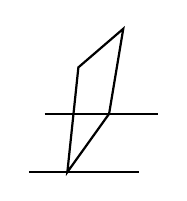
\begin{tikzpicture}[x=1cm,y=1cm,line width=.8pt]
\draw (-.2,0)--(1.2,0); \draw (0,.74)--(1.44,.74);
\draw (.29,0)--(.43,1.33)--(1,1.82)--(.82,.74)--cycle;
\end{tikzpicture}}

\figure{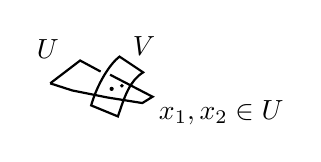
\begin{tikzpicture}[x=1cm,y=1cm,line width=.8pt]
\draw (0,.55)--(.38,.84)--(.64,.70) (.76,.66)--(1.3,.38)--(1.17,.30)--(.73,.37)--(.28,.46)--(0,.55);
\draw (.52,.27) .. controls (.60,.55) and (.76,.80) .. (.88,.89)--(1.18,.69) .. controls (1.01,.58) and (.95,.40) .. (.86,.13)--cycle;
\fill (.78,.48) circle (.027); \fill (.91,.52) circle (.025);
\node at (-.03,.98) {$U$};\node at (1.19,1.02) {$V$};\node[anchor=west] at (1.25,.18) {$x_1,x_2\in U$};
\end{tikzpicture}}

\diagram{\begin{tikzcd}[ampersand replacement=\&,row sep=small,column sep=small]
X(1)\arrow[dr,bend right=12]\&\&X(2)\arrow[dl,bend left=12]\\
\&Y\&
\end{tikzcd}}

\[
\begin{aligned}
&\dim X=3\quad\dim Y=4\\
&\dim F_3=1\\
&\dim\alpha_{ij}(\overline F_{\unsure{2|1}})=2
\end{aligned}
\]

